\glsresetall
% Implementation Process -------------------------------------------------------------------------
\chapter{Implementation Process}
\label{chap:implementation_process}

This chapter presents the implementation process of the proposed solution explained in the previous chapter. Every step is explained taking into consideration the most important points to implement the methods. This chapter covers three main sections: First, \ref{sec:data_set} - \nameref{sec:data_set}, the data provided to perform this research is briefly exposed and analysed. Second, \ref{sec:metrics_gathering} - \nameref{sec:metrics_gathering}, the implementation of Graphy (\gls{otp}), our proposed solution to collect metrics from tracing data presented in the chapter \ref{chap:possible_solution}, is explained in detail. Finally, \ref{sec:observations_analysis} - \nameref{sec:observations_analysis}, the methods for analysis of the stored observations are presented with the respective results and answers to the research questions.

\section{Huawei Tracing Data Set}
\label{sec:huawei_tracing_data_set}

Nothing comes from nothing, and in this project the starting point for every method developed was a data set provided by Huawei, represented by professor Jorge Cardoso. To be able to get access to this information, a NDA: Non-disclosure agreement were signed by both parts. This data set contains the results of tracing data gathered from an experimental cluster used by the company for testing purposes. In terms of time this data is a representation of two days of the systems workload, therefore two files were provided, one for each day. These files were generated in 2018-07-10 and for protection, some fields of the data set were obfuscated during the generation process.

\begin{table}[H]
\caption{Data set provided for this research.}
\label{table:data_set_provided_for_this_research}
\centering
\large
\begin{tabularx}{\linewidth} {
    |>{\hsize=0.70\hsize}X| 
     >{\hsize=1.15\hsize}X|
     >{\hsize=1.15\hsize}X| }
     \hline
    
    & 2018-06-28
    & 2018-06-29 \\ \hline
    \textbf{File}
    & traces-2018-06-28.jsonl
    & traces-2018-06-29.jsonl \\ \hline
    % \textbf{Size}
    % & 130 megabytes
    % & 164 megabytes \\ \hline
    \textbf{Spans count}
    & 190 202
    & 239 693 \\ \hline
    \textbf{Traces count}
    & 64 394
    & 74 331 \\ \hline
\end{tabularx}
\end{table}

As we can see by the information presented in the table \ref{table:data_set_provided_for_this_research}, each file represents a day of traces and both were written in JSONL format \cite{jsonl}. This type of file format is an extension to the normal lightweight data-interchange standard JSON: JavaScript Object Notation file type, however, in JSONL multiple JSONs are separated by a new line character. Each Span is presented by a single JSON, so for each line we have a Span encoded in JSON format. Further in this sections is a representations of the amount of traces by hour, to do this and to perform the traces count we have to map the span trees, the explanation and algorithm are presented in the next section \ref{sec:metrics_gathering} - \nameref{sec:metrics_gathering}.

Span data format is defined in a specification, but companies and software developers do not need to strictly follow it, they can produce their own span data format and this means that each software company can have their own span specification. To ensure the understanding and follow up with the span data format, there was a file with instructions about the spans. In this file, the fields were explained, this consisted in their specific names and the supposed data type. A brief sample of the explanation provided in the file is exposed in the points bellow.

\begin{enumerate}[topsep=1pt, partopsep=1pt, itemsep=5pt, parsep=5pt]
    \item traceId - Unique id of a trace (128-bit string).
    \item name - Human-readable title of the instrumented function.
    \item timestamp - UNIX epoch in milliseconds.
    \item id - Unique id of the span (64-bit string).
    \item parentId - Reference to id of parent span.
    \item duration - Span duration in microseconds.
    \item binaryAnnotations:
    \begin{enumerate}[topsep=1pt, partopsep=1pt, itemsep=5pt, parsep=5pt]
        \item protocol - 'HTTP' or 'function' for RPC calls.
        \item http.url - HTTP endpoint.
        \item http.status\textunderscore code - Result of the HTTP operation. 
    \end{enumerate}
    \item annotations:
    \begin{enumerate}[topsep=1pt, partopsep=1pt, itemsep=5pt, parsep=5pt]
        \item value - Describes the position in trace (based on Zipkin format). Could be one of the following values or other: 'cs' (client send), 'cr' (client receive), 'ss' (server send) or 'sr' (server receive)
        \item timestamp - UNIX epoch in microseconds.
        \item endpoint - Wich endpoint generated a trace event.
    \end{enumerate}
\end{enumerate}

Two notes were also provided within this file. To point each one, has they are very important, we present them bellow.

\begin{enumerate}[topsep=1pt, partopsep=1pt, itemsep=5pt, parsep=5pt]
    \item Time units are not consistent, some fields are in milliseconds and some are in microseconds.
    \item Trace spans may contain more fields, except those mentioned here.
\end{enumerate}

From the point presented above, we get a notion that we need to consider some things about the values that we might encounter in the spans fields. Some fields are required by the OpenTracing specification as presented in \ref{subsec:distributed_tracing}, and to sanitise this whole topic, it is very important that a company, when producing this kind of information, stick with the specification, even if it is an open-source specification. So "traceId", "name", "timestamp", "id" and "parentId" are required fields, this is because they are the foundations to identify a span, produce relation between them and to place them in time. Other topic that is very important to understand is that the specification is not precise, we do not know clearly what is available when working with a span, this means that there is no specific data structure for fields like "binaryAnnotations" and "annotations", and this is a big problem as we might have spans that are completed or incomplete and we can not know it as there is nothing to tell us about it. For example, in the "binaryAnnotations" the information is disposed in key value objects, and as said in the second point of the notes presented above: "Trace spans may contain more fields, except those mentioned here", this causes a tremendous explosion in possibilities, because there might be keys with their corresponding values for some particular spans and it gets hard to generalise this whole span structure.

At the current time of writing, the clarity of span data only depends if the company that produced the software or the software owner care about what the system will produce in terms of tracing data. To be sure that the teams developing distributed software produce good tracing data, the company must implement a standard for every team to follow. The normalisation and unification of the span format should be one thing to consider in the near future, this is because it is very hard to perceive and distinguish multiple span types. For example, in the data provided spans can be of two types: \gls{http} Span or \gls{rpc} Span, and the only field that distinguishes them is that the second one has an "exec" field, which stands for the execution process id, and that is not presented in the HTTP span type. Another example, for the measure units of some fields, if the field have the same key, they all should be in one single measure unit, this is because some tools are expecting this, and they assume wrong values when spans have time-stamps in milliseconds and others in microseconds like in this case.

To give a brief notion of how the traces and spans are spread throughout time, we have used our tool, \todo{Graphy \gls{otp}}, to generate two charts that represents the counting of traces and spans for each hour in each day. The decision to generate two spitted charts comes from the simple fact that we have one file for each day. To be able to count the spans in time, in this case by hour, the tool only needs to group every span by hour and count them, however for traces, the tool has a lot more work has it have to merge all spans in their corresponding trace (explained in \ref{sec:metrics_gathering}. After having all traces, we can count them like we count spans. Note that if a span or trace starts at a given time (t1) contained in a time-frame (tf1), and with its duration (d1) surpasses the next time-frame (tf2), (t1 + d1 \textgreater tf2), it is considered to be in the tf1, or by other words, only the starting time of the trace or span is considered for the counting. The figures \ref{fig:trace_file_count_2018_06_28} and \ref{fig:trace_file_count_2018_06_29} presents the data set traces and spans counting throughout time.

\begin{figure}[H]
    \centering
    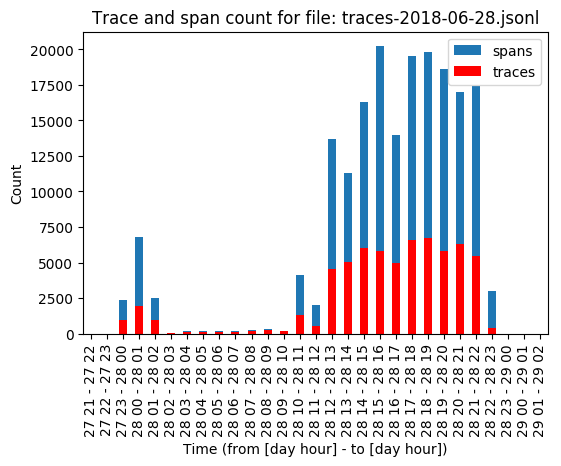
\includegraphics[width=0.88\textwidth]{images/trace_file_count_2018_06_28_chart.png}
    \caption{Trace file count for 2018-06-28.}
    \label{fig:trace_file_count_2018_06_28}
\end{figure}

\begin{figure}[H]
    \centering
    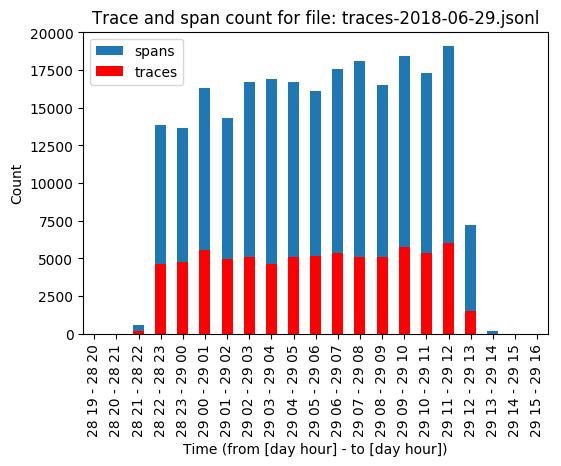
\includegraphics[width=0.88\textwidth]{images/trace_file_count_2018_06_29_chart.png}
    \caption{Trace file count for 2018-06-29.}
    \label{fig:trace_file_count_2018_06_29}
\end{figure}

// A big region without traces, why? Can't answer that!

// Less data spreaded through time than the previous one.

// Maybe include here the Quality of tracing analysis and possibilities in their own analysis.


\section{Open Tracing Processor Component}
\label{sec:open_tracing_processor_component}

\todo{Start by explaining how the metrics relate with the questions, and what metrics we decided to extract and were, how do we put it there.

Explain how to map spans into span trees.
to process the information presented in the data set and store it for our own analysis purposes

... as explained in \ref{subsec:traces_and_spans}, each spans relates with another, in this case, by a field called parent id. After mapping the spans into trees, we end up with a list of tress, each for a specific trace, and we just have to count them. To map the spans into trees, we index it by the 

// TODO: Regarding database setup and implementations, the choices were to use OpenTSDB as a Time-Series database and ArangoDB as a graph database. However, the second choice wasn't the better one, due to some lack of support and terrible \gls{api} documentation. Some issues were opened in the GitHub client \gls{api} for the programming language Python, but the answer was always that it have the expected behaviour \cite{arango_issues}. This have lead to some difficulties when implementing the component Graphs Repository, presented in Graphy API. Some difficulties were felted when trying to store graphs with custom names and setting up different type values to some data structures presented in the pyArango client API. The solution was to fetch all the API, perform some changes and use our custom pyArango client. This changes were committed for review to the original project stored on GitHub. Mitigating this kind of problems was something that was impossible to predict when choosing the Graph storing technology.}

\begin{algorithm}[H]
\SetAlgoLined
\KwResult{Write here the result }
 initialization\;
 \While{While condition}{
  instructions\;
  \eIf{condition}{
   instructions1\;
   instructions2\;
   }{
   instructions3\;
  }
 }
 \caption{How to write algorithms}
\end{algorithm}

\todo{aaa}

// Finally present the display of information in the Grafana with some prints. Refer that the lack of data in day 28. And do some observations. 

% Observations Analysis --------------------------------------------------------------------------
\section{Data Analysis Component}
\label{sec:data_analysis_component}

// TODO: Talk about Unlabeled data, the best algorithms to handle this kind of situation and how we did it.


%-------------------------------------------------------------------------------------------------


%-------------------------------------------------------------------------------------------------
\checkoddpage
\ifthenelse{\boolean{oddpage}}
{ % Odd page
\newpage
\blankpage}
{ % Even page
}
%-------------------------------------------------------------------------------------------------